\documentclass[aspectratio=169]{beamer}
\usetheme{Madrid}
\usecolortheme{default}
\usepackage[utf8]{inputenc}
\usepackage[T5]{fontenc}
\usepackage{graphicx}
\usepackage{hyperref}
\usepackage{booktabs}

\setbeamertemplate{caption}[numbered]
\renewcommand{\figurename}{Hình}

\title[Buổi 1 TH: AI \& Prompting]{Thực hành AI Tạo sinh (GAI) trong Kế toán \\ \vspace{0.3cm} \Large Buổi 1: Kỹ năng Prompt cơ bản}
\author{Đại học Đông Á}
\date{\today}

\begin{document}

% SLIDE 1
\begin{frame}
    \titlepage
    \begin{center}
        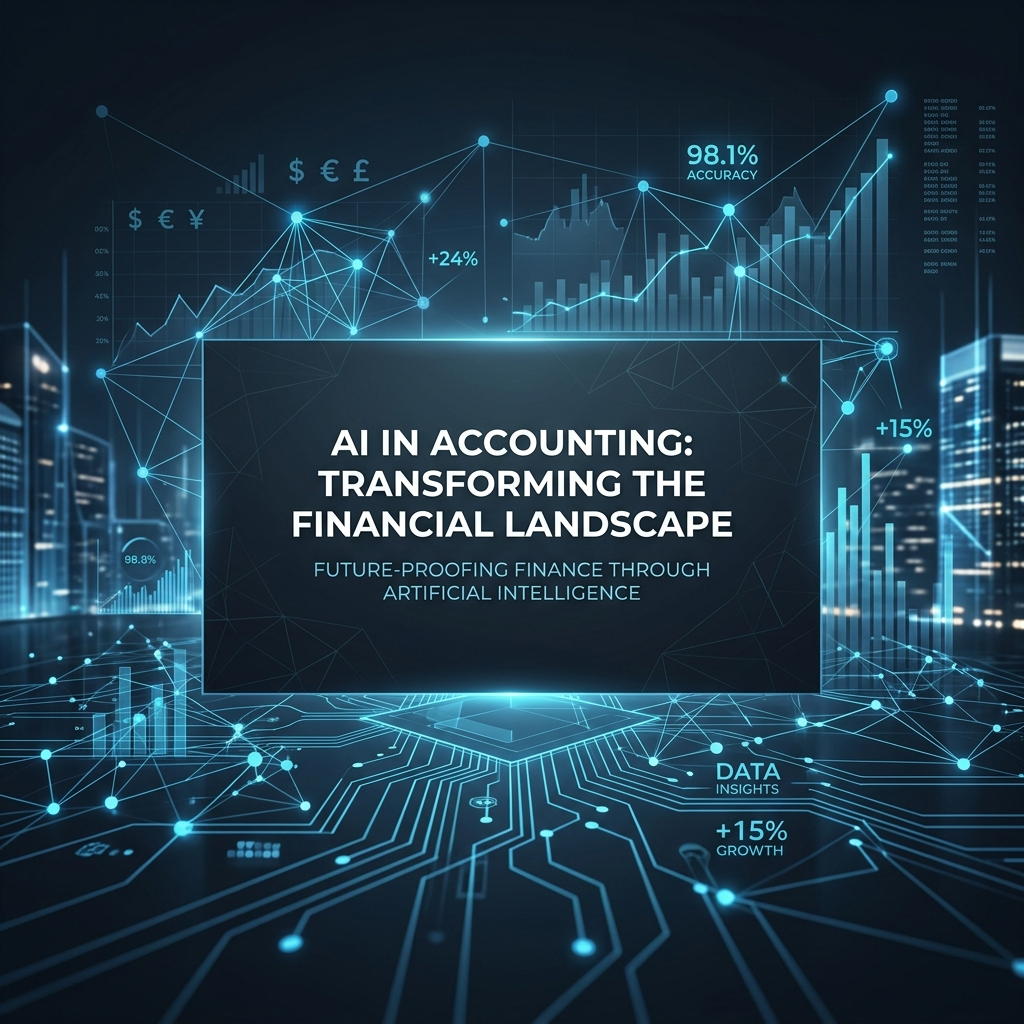
\includegraphics[width=0.5\textwidth,height=2.5cm,keepaspectratio]{images/Day_01_TH/bg_tech.png}
    \end{center}
\end{frame}

% SLIDE 2
\begin{frame}{Nội dung Chương trình Thực hành}
    \tableofcontents
\end{frame}

% SLIDE 3
\begin{frame}{Khởi động (Ice-breaker)}
    \begin{quote}
        \textit{"Nó chậm, nhiều lỗi, làm nhiều thứ chưa tốt, nhưng những chiếc máy tính đầu tiên cũng vậy."} \\
        \vspace{0.3cm}
        \raggedleft -- \textbf{Sam Altman, OpenAI CEO} --
    \end{quote}
    \vspace{0.5cm}
    \textbf{Thông điệp:} \\
    Đừng kỳ vọng AI hoàn hảo ngay lập tức. Kế toán viên cần học cách dùng nó từ bây giờ để không bị bỏ lại phía sau.
\end{frame}

% SLIDE 4
\begin{frame}{Năng lực đạt được sau buổi học}
    \begin{itemize}
        \item \textbf{Về Lý thuyết (LT):} Nắm vững nền tảng Hệ thống Thông tin Kế toán (AIS); Phân biệt rõ sự khác nhau giữa AI, Machine Learning và Deep Learning trong bối cảnh kế toán tài chính.
        \item \textbf{Về Thực hành (TH):} Có khả năng sử dụng các Generative AI (ChatGPT, Copilot, Gemini) để đóng vai (Role-play) hỗ trợ giải đáp các chuẩn mực kế toán cơ bản.
        \item \textbf{Về Tư duy nghề nghiệp:} Chấp nhận và thích nghi với sự thay đổi của nghề kế toán trong kỷ nguyên AI; Nhận thức AI là công cụ hỗ trợ (Copilot), không phải mối đe dọa thay thế hoàn toàn kế toán viên.
    \end{itemize}
\end{frame}

\section{1. Điều kiện tiên quyết \& Công cụ AI kế toán}

% SLIDE 5
\begin{frame}{Điều kiện tiên quyết (Prerequisites)}
    Để áp dụng hiệu quả AI trong công việc, hạ tầng kỹ thuật không cần quá phức tạp nhưng phải đúng chuẩn.
    \vspace{0.3cm}
    \\
    Gồm 3 khía cạnh chính:
    \begin{enumerate}
        \item Trình duyệt Web hiện đại.
        \item Quyền truy cập Nền tảng AI.
        \item Tư duy học hỏi mở.
    \end{enumerate}
\end{frame}

% SLIDE 6
\begin{frame}{Công cụ cần có: Phần mềm \& Tài khoản}
    \begin{columns}
        \column{0.5\textwidth}
        \begin{itemize}
            \item \textbf{Trình duyệt web hiện đại:} Chrome, Edge, Safari.
            \item \textbf{Quyền truy cập Nền tảng AI:}
            \begin{itemize}
                \item Đăng ký tài khoản OpenAI (ChatGPT)
                \item Hoặc Google Gemini
            \end{itemize}
        \end{itemize}
        \column{0.5\textwidth}
        \centering
        
\includegraphics[width=0.8\textwidth,height=3cm,keepaspectratio]{images/Day_01_TH/chatgpt_logo.png}
    \end{columns}
\end{frame}

% SLIDE 7
\begin{frame}{Tư duy cần có: Sự tò mò trí tuệ}
    \begin{center}
        \Large \textbf{Intellectual Curiosity}
    \end{center}
    \vspace{0.5cm}
    \begin{itemize}
        \item Vượt qua rào cản kỹ thuật.
        \item Cần một tư duy cởi mở để \textbf{khám phá, thử nghiệm (experiment)} và thích nghi.
        \item Máy móc sẽ xử lý dữ liệu, con người sẽ đặt câu hỏi!
    \end{itemize}
\end{frame}

% SLIDE 8
\begin{frame}{Hệ sinh thái Phần mềm Kế toán tích hợp AI}
    \begin{columns}
        \column{0.6\textwidth}
        \begin{itemize}
            \item \textbf{Xử lý dữ liệu tự động:} QuickBooks, Xero.
            \item \textbf{Phân tích \& Báo cáo nâng cao:} IBM Cognos Analytics, Tableau.
            \item \textbf{Lưu trữ đám mây \& Bảo mật:} AWS, Microsoft Azure.
        \end{itemize}
        \column{0.4\textwidth}
        \centering
        
\includegraphics[width=0.45\textwidth]{images/Day_01_TH/quickbooks_logo.png} 
        
\includegraphics[width=0.45\textwidth]{images/Day_01_TH/xero_logo.png} \\
        \vspace{0.2cm}
        
\includegraphics[width=0.45\textwidth]{images/Day_01_TH/tableau_logo.png} 
        
\includegraphics[width=0.45\textwidth]{images/Day_01_TH/aws_logo.png}
    \end{columns}
\end{frame}

\section{2. Ứng dụng AI Tự động hóa \& Phân tích dự báo}

% SLIDE 9
\begin{frame}{Đột phá của AI trong Tính toán Kế toán}
    AI không chỉ tính toán cộng trừ nhân chia, mà xử lý các \textbf{kịch bản tài chính cực kỳ phức tạp}.
    \vspace{0.5cm}
    \\
    Tập trung vào 2 trụ cột chính:
    \begin{enumerate}
        \item Tự động hóa tính toán (Automating Calculations).
        \item Phân tích dự báo (Predictive Analytics).
    \end{enumerate}
\end{frame}

% SLIDE 10
\begin{frame}{Tự động hóa các tính toán phức tạp}
    \begin{itemize}
        \item \textbf{Hiệu suất và chính xác:} Tự động tính thuế, khấu hao, dự phóng tài chính với tốc độ đáng kinh ngạc.
        \item \textbf{Thuật toán thích ứng (Adaptive algorithms):} AI liên tục học luật thuế mới, cập nhật chuẩn mực (IFRS/VAS) để tuân thủ kịp thời.
    \end{itemize}
\end{frame}

% SLIDE 11
\begin{frame}{Giảm thiểu sai sót (Error Reduction)}
    \begin{columns}
        \column{0.5\textwidth}
        \begin{itemize}
            \item \textbf{Tác động:} Loại bỏ rủi ro do con người mệt mỏi, nhập sai số liệu.
            \item Đảm bảo tính tuân thủ pháp lý khắt khe.
        \end{itemize}
        \column{0.5\textwidth}
        \centering
        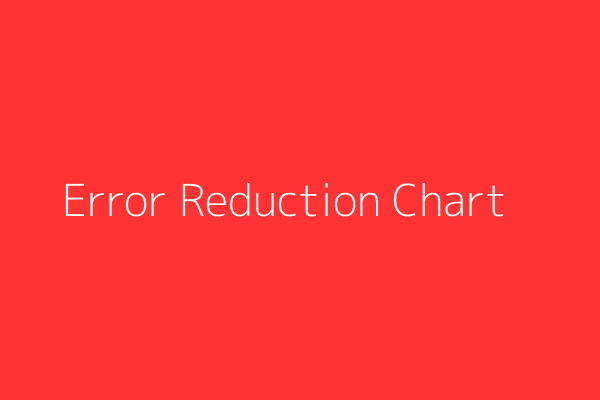
\includegraphics[width=0.9\textwidth]{images/Day_01_TH/error_reduction.png}
    \end{columns}
\end{frame}

% SLIDE 12
\begin{frame}{Khả năng Phân tích Dự báo (Predictive Analytics)}
    \begin{itemize}
        \item \textbf{Dự báo (Forecasting):} Dựa trên dữ liệu lịch sử để vẽ ra các kịch bản dòng tiền tương lai.
        \item \textbf{Hỗ trợ Quyết định:} Hỗ trợ lãnh đạo ra quyết định chiến lược thay vì chỉ nhìn vào báo cáo quá khứ tĩnh.
    \end{itemize}
\end{frame}

% SLIDE 13
\begin{frame}{Phân tích \& Diễn giải Dữ liệu (Data Interpretation)}
    Không chỉ xử lý số liệu, AI có khả năng \textbf{"đọc vị" dữ liệu}:
    \begin{itemize}
        \item \textbf{Nhận diện xu hướng (Trends):} Mùa vụ kinh doanh, thay đổi sở thích.
        \item \textbf{Phát hiện rủi ro tiềm ẩn (Risks):} Cảnh báo công nợ khó đòi sớm.
        \item \textbf{Tối ưu hóa lợi nhuận:} Chỉ ra các khu vực lãng phí chi phí.
    \end{itemize}
\end{frame}

% SLIDE 14
\begin{frame}{Lời khuyên Tài chính Cá nhân hóa}
    \begin{itemize}
        \item AI không đưa ra lời khuyên chung chung kiểu "sách giáo khoa".
        \item Nó tùy chỉnh chiến lược dựa trên bối cảnh đặc thù của từng doanh nghiệp:
        \begin{itemize}
            \item Ngành nghề kinh doanh.
            \item Quy mô hiện tại.
            \item Tình trạng dòng tiền thực tế.
        \end{itemize}
    \end{itemize}
\end{frame}

\section{3. Case Studies - Bài toán thực tế}

% SLIDE 15
\begin{frame}{Tại sao cần Case Study?}
    Học qua thực tiễn: Xem cách AI tháo gỡ khó khăn cho các quy mô doanh nghiệp khác nhau:
    \begin{itemize}
        \item \textbf{Doanh nghiệp siêu nhỏ:} Quán cà phê Brewed Awakenings.
        \item \textbf{Doanh nghiệp vừa:} Công ty tư vấn thiết kế Cityscape Consulting.
        \item \textbf{Tập đoàn Đa quốc gia:} GlobalTech Enterprises.
    \end{itemize}
\end{frame}

% SLIDE 16
\begin{frame}{Case Study 1: Quán cà phê Brewed Awakenings}
    \begin{columns}
        \column{0.6\textwidth}
        \begin{itemize}
            \item \textbf{Bối cảnh:} Cửa hàng cà phê nhỏ, ít nhân sự. Đau đầu vì quản lý chi phí, tính thuế và dòng tiền lẻ tẻ mỗi ngày.
            \item \textbf{Giải pháp:} Sử dụng phần mềm \textbf{QuickBooks Online} có tích hợp AI.
        \end{itemize}
        \column{0.4\textwidth}
        \centering
        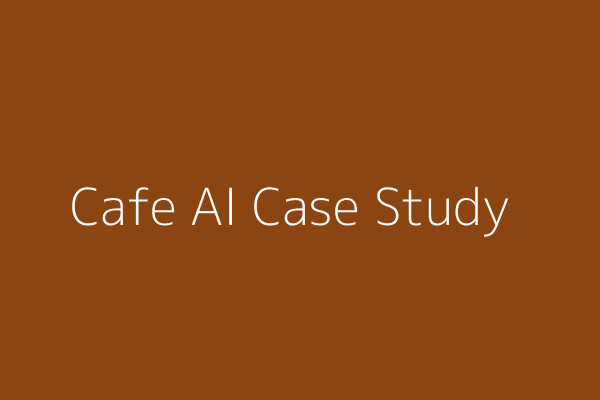
\includegraphics[width=0.9\textwidth]{images/Day_01_TH/cafe_ai.png}
    \end{columns}
\end{frame}

% SLIDE 17
\begin{frame}{Kết quả tại Brewed Awakenings}
    \begin{itemize}
        \item Phân loại tự động chi phí (Categorization) từ hóa đơn đầu vào.
        \item Đồng bộ giao dịch ngân hàng theo thời gian thực (Bank Feeds).
        \item \textbf{Thành quả lớn nhất:} Dự báo dòng tiền \& Lập kế hoạch thuế. Chủ quán hoàn toàn rảnh tay để tập trung chăm sóc khách hàng.
    \end{itemize}
\end{frame}

% SLIDE 18
\begin{frame}{Case Study 2: Cityscape Consulting}
    \begin{columns}
        \column{0.6\textwidth}
        \begin{itemize}
            \item \textbf{Bối cảnh:} Công ty tư vấn kiến trúc. Ngân sách từng dự án thiết kế thay đổi liên tục, cần quản lý chi phí sát sao.
            \item \textbf{Giải pháp:} Áp dụng \textbf{Xero AI}.
        \end{itemize}
        \column{0.4\textwidth}
        \centering
        
\includegraphics[width=0.9\textwidth]{images/Day_01_TH/architecture_ai.png}
    \end{columns}
\end{frame}

% SLIDE 19
\begin{frame}{Kết quả tại Cityscape Consulting}
    \begin{itemize}
        \item Theo dõi sức khỏe tài chính dự án (Real-time overview).
        \item AI gợi ý các cơ hội tiết kiệm chi phí mua sắm vật liệu và các khoản được khấu trừ thuế mảng dịch vụ.
        \item \textbf{Thành quả:} Biến phần mềm Xero thành "Giám đốc tài chính ảo" (Virtual CFO).
    \end{itemize}
\end{frame}

% SLIDE 20
\begin{frame}{Nhìn lại Doanh nghiệp vừa \& nhỏ (SMEs)}
    \begin{center}
        \Large \textbf{AI đã san bằng sân chơi (Leveling the playing field)}
    \end{center}
    \vspace{0.5cm}
    Các doanh nghiệp nhỏ giờ đây có trong tay sức mạnh phân tích tài chính cực kỳ chuyên sâu -- thứ mà trước đây vốn chỉ dành cho các tập đoàn lớn có ngân sách CNTT hàng triệu USD!
\end{frame}

% SLIDE 21
\begin{frame}{Case Study 3: Tập đoàn GlobalTech Enterprises}
    \begin{columns}
        \column{0.6\textwidth}
        \begin{itemize}
            \item \textbf{Bối cảnh:} Tập đoàn đa quốc gia. Chi nhánh ở nhiều quốc gia, phải tuân thủ hàng chục luật thuế khác nhau (VAT, GST, State Tax).
            \item \textbf{Giải pháp:} Tích hợp \textbf{IBM Watson} (Hệ thống AI doanh nghiệp).
        \end{itemize}
        \column{0.4\textwidth}
        \centering
        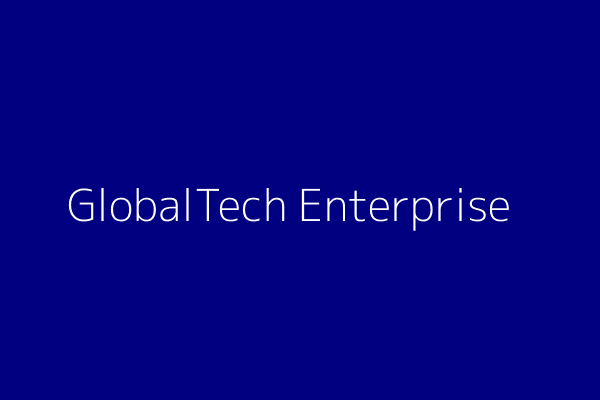
\includegraphics[width=0.9\textwidth]{images/Day_01_TH/global_ai.png}
    \end{columns}
\end{frame}

% SLIDE 22
\begin{frame}{Sức mạnh của IBM Watson tại GlobalTech}
    \begin{itemize}
        \item Tự động hóa tuân thủ thuế quốc tế (Automated international compliance).
        \item \textbf{Mô hình hóa tài chính dự báo toàn cầu (Predictive modeling):} Đối phó với tỷ giá hối đoái, lạm phát.
        \item Xử lý mượt mà hàng triệu hóa đơn chuyển giá liên công ty (Inter-company transfers).
    \end{itemize}
\end{frame}

% SLIDE 23
\begin{frame}{Bài toán Đạo đức \& Bảo mật tại Tập đoàn lớn}
    \begin{itemize}
        \item \textbf{Rủi ro lớn nhất:} Lộ lọt dữ liệu nhạy cảm tài chính.
        \item \textbf{Giải pháp:} IBM Watson được tinh chỉnh để tuân thủ nghiêm ngặt chuẩn \textbf{GDPR} (Châu Âu) và \textbf{CCPA} (Mỹ).
        \item \textbf{Kiểm toán liên tục (Continuous Audits):} Kiểm tra chéo ngay cả đối với chính hệ thống AI.
    \end{itemize}
\end{frame}

% SLIDE 24
\begin{frame}{Tính công bằng của AI (Bias and Fairness)}
    \begin{itemize}
        \item \textbf{Sự minh bạch (Transparency):} Con người phải hiểu được tại sao AI đưa ra quyết định đó.
        \item \textbf{Tính công bằng:} Đảm bảo AI không mang định kiến (bias) khi chấm điểm tín dụng khách hàng hoặc phê duyệt nhà cung cấp dựa trên khu vực địa lý, xuất thân.
    \end{itemize}
\end{frame}

\section{4. Chuẩn bị Kỹ năng \& Hướng dẫn Prompt}

% SLIDE 25
\begin{frame}{Chuẩn bị cho Tương lai AI (Future-proofing)}
    \begin{center}
        \textit{"Máy móc không thay thế con người, nhưng người dùng máy móc sẽ thay thế người không dùng máy."}
    \end{center}
    \vspace{0.5cm}
    Giới thiệu \textbf{5 Kỹ năng cốt lõi} mà Kế toán viên cần trang bị ngay hôm nay để tồn tại trong kỷ nguyên mới.
    \begin{center}
        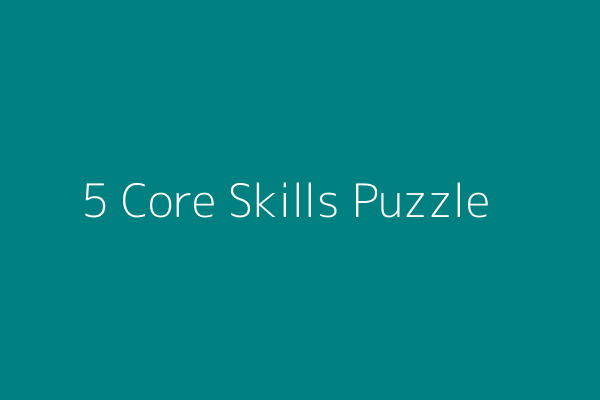
\includegraphics[width=0.4\textwidth]{images/Day_01_TH/puzzle_skills.png}
    \end{center}
\end{frame}

% SLIDE 26
\begin{frame}{Kỹ năng 1: Hiểu biết về AI (AI Literacy)}
    \begin{itemize}
        \item Không yêu cầu phải biết lập trình thuật toán Python/C++.
        \item Phải hiểu cách AI hoạt động cơ bản (Input $\rightarrow$ Blackbox $\rightarrow$ Output).
        \item Nắm vững các khái niệm Học máy (Machine Learning) để biết được "AI có thể làm gì và KHÔNG thể làm gì".
    \end{itemize}
\end{frame}

% SLIDE 27
\begin{frame}{Kỹ năng 2: Quản lý Dữ liệu (Data Proficiency)}
    \begin{itemize}
        \item \textbf{Data Quality:} Đảm bảo nguồn dữ liệu cung cấp cho AI là dữ liệu sạch. Rác vào thì rác ra.
        \item \textbf{Data Interpretation:} Kỹ năng diễn giải đầu ra của AI. Biến các báo cáo khô khan của máy thành các chiến lược hành động cụ thể cho con người.
    \end{itemize}
\end{frame}

% SLIDE 28
\begin{frame}{Kỹ năng 3 \& 4: Công nghệ và Phản biện}
    \begin{itemize}
        \item \textbf{Kỹ năng 3 - Am hiểu Công nghệ:} 
        \begin{itemize}
            \item Nắm bắt giao diện và luồng làm việc của các ERP tích hợp AI (QuickBooks, Xero).
            \item Khả năng thích ứng cao khi giao diện phần mềm cập nhật liên tục.
        \end{itemize}
        \item \textbf{Kỹ năng 4 - Tư duy Phản biện:}
        \begin{itemize}
            \item AI đưa ra số liệu, con người ra Quyết định cuối cùng.
            \item Phải biết Fact-checking (tra cứu chéo) số liệu do AI tạo ra để tránh "ảo giác" tài chính.
        \end{itemize}
    \end{itemize}
\end{frame}

% SLIDE 29
\begin{frame}{Kỹ năng 5: Học tập suốt đời (Continuous Learning)}
    \begin{itemize}
        \item Công nghệ AI và Thuế thay đổi từng ngày.
        \item Một kỹ năng học được hôm nay có thể hoàn toàn lỗi thời vào tháng sau.
        \item Yêu cầu: Liên tục tham gia các hội thảo, diễn đàn, khóa học cập nhật FinTech \& AI.
    \end{itemize}
\end{frame}

% SLIDE 30
\begin{frame}{LAB 1: Khởi động với ChatGPT (Prompting 101)}
    \begin{columns}
        \column{0.5\textwidth}
        \textbf{Nhiệm vụ 1:} Đăng nhập vào ChatGPT / Gemini.
        \vspace{0.3cm}
        \\
        \textbf{Thực hành viết Prompt cơ bản:} \\
        \textit{"Hãy đóng vai một chuyên gia Kế toán, giải thích cho tôi khái niệm 'Khấu hao theo đường thẳng' bằng ngôn ngữ đơn giản cho người không chuyên."}
        \column{0.5\textwidth}
        \centering
        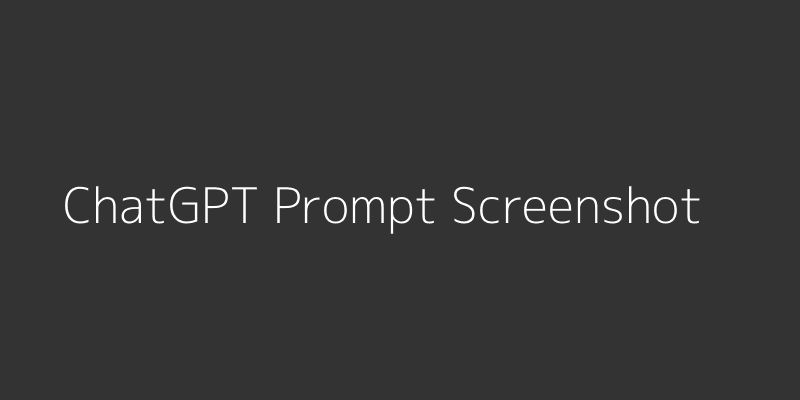
\includegraphics[width=0.9\textwidth]{images/Day_01_TH/prompt_screenshot.png}
    \end{columns}
\end{frame}

% SLIDE 31
\begin{frame}{LAB 2: Xử lý tình huống Kế toán}
    \textbf{Nhiệm vụ:} Dùng AI viết một email nhắc nợ chuyên nghiệp.
    \vspace{0.3cm}
    \begin{itemize}
        \item \textbf{Thử nghiệm 1 (Prompt chung chung):} "Viết email đòi nợ khách hàng." 
        \item $\rightarrow$ \textit{Kết quả: Nội dung thường cộc lốc, không chuyên nghiệp.}
        \item \textbf{Thử nghiệm 2 (Prompt tối ưu):} "Đóng vai Kế toán công nợ, viết 1 email lịch sự nhưng kiên quyết đòi khoản nợ 50 triệu đã quá hạn 30 ngày từ công ty XYZ. Văn phong chuyên nghiệp, ngụ ý sẽ tính lãi trả chậm."
        \item $\rightarrow$ \textit{Kết quả: Hoàn toàn khác biệt, xuất sắc.}
    \end{itemize}
\end{frame}

% SLIDE 32
\begin{frame}{Tổng kết Buổi Thực hành}
    \begin{itemize}
        \item Các công cụ phần mềm (QuickBooks, Xero, IBM Watson) đang định hình lại toàn bộ cách kế toán vận hành từ SME đến Tập đoàn lớn.
        \item Hành trang mang về: 
        \begin{enumerate}
            \item Tư duy và 5 Kỹ năng sinh tồn kỷ nguyên mới.
            \item Kỹ thuật đặt câu lệnh (Prompting) đầu tiên.
        \end{enumerate}
    \end{itemize}
\end{frame}

% SLIDE 33
\begin{frame}{Q\&A \& Hướng dẫn Tự học}
    \begin{center}
        \Large \textbf{Hỏi \& Đáp (Q\&A)}
    \end{center}
    \vspace{0.5cm}
    \textbf{Bài tập về nhà:} \\
    Hãy tạo một kịch bản Prompt cho ChatGPT để yêu cầu nó tóm tắt một đoạn quy định thuế dài 3 trang thành 5 gạch đầu dòng dễ hiểu. 
    Lưu lại kết quả và nộp vào buổi sau!
\end{frame}

% SLIDE 34
\begin{frame}
    \begin{center}
        \Huge \textbf{Thank You!} \\
        \vspace{1cm}
        \normalsize Hẹn gặp lại vào Buổi 2.
    \end{center}
\end{frame}

\end{document}
